\section{RNASeq}

\subsection{Introduction}

\subsection{Methods}

\subsubsection{GO Term Distributions}

\begin{figure}[H]
  \centering
  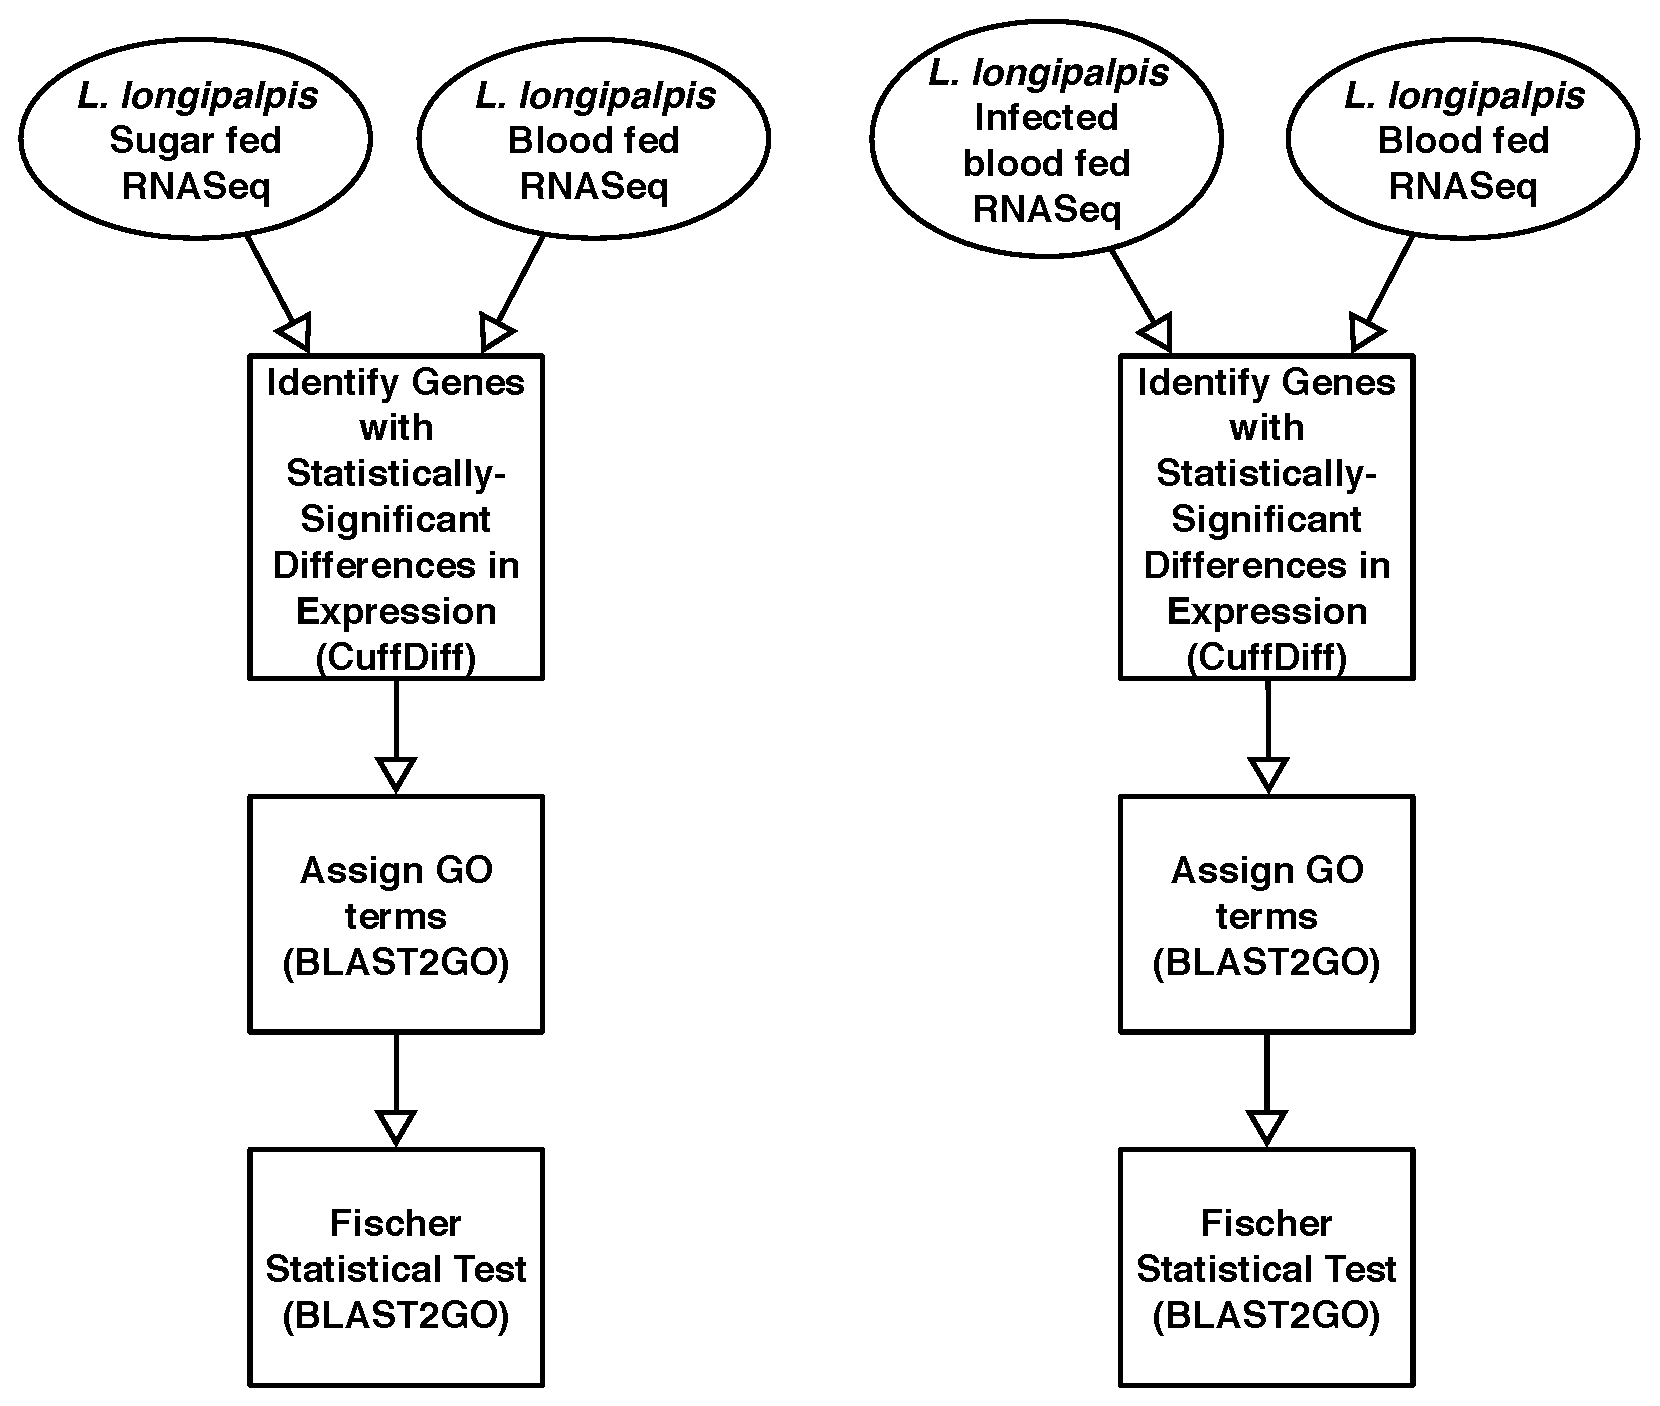
\includegraphics[width=0.7\textwidth]{figures/rnaseq/cuffdiff_workflow}
  \caption{Workflow for Comparing Gene Expression}
  \label{fig:rnaseq-cuffdiff-workflow}
\end{figure}

\textcolor{red}{TODO Cuffdiff}

Gene identifiers for genes marked as statistically significant by \texttt{CuffDiff} were extracted for each time point and feeding condition.  The corresponding protein sequences for each gene were extracted from the genomes.  The protein sequences were merged and run through \texttt{BLAST2GO}. \textcolor{red}{TODO CITE, VERSION}

\subsection{Results}

\subsubsection{Analysis of RNASeq Assemblies}

\subsubsection{GO Term Distribution Differences}

\begin{table}[H]
  \centering
  \begin{tabular}{c c c} \hline
  \emph{Time Point} & \emph{Blood Fed vs Sugar Fed} & \emph{Infected Blood Fed vs Blood Fed} \\ \hline
  6H & 3,111 & 271 \\ \hline
  24H & 4,120 & 658 \\ \hline
  144H & 4,571 & 290 \\ \hline
  \end{tabular}
  \caption{Number of Genes with Statistically-Significant Differential Expression}
  \label{tab:stat-sig-genes}
\end{table}

\subsubsection{Pathway Analysis}

\subsubsection{Differential Expression by Gene Family}


\subsection{Discussion and Conclusion}